\section{Exchange Transactions and Errors}
\label{section:exchange_transactions_and_errors}

% A back-of-an-envelope calculation reveals that within an order of magnitude this hypothesis results
% in all the variables reacting with each other within an orderin a way we have observed in economic
% systems. An error rate of 5 percent is maybe reasonable. An error rate of 10 percent seems
% unreasonably large. From personal experience visiting a supermarket, there is some chance that a
% line of goods we were expecting to buy is not available. This is probably less than 1 in every 10
% purchases we are expecting to make. On the other hand 1 percent probably seems too small, though not
% impossible. Communication systems typically require 2.5 - 10 times the error rate to expend to
% compensate for errors, so we could assume a reasonable number is 5. The hypothesis implies that an
% increase in the growth rate  1 percent increase in the growth rate will cause a 1 in 5 percent
% increase the unemployment rate for a given inflation rate. This is certainly in the right direction
% but seems a little small. Unemployment rates typically fluctuate between 3 and 10 percent, but to
% drive a reduction in the unemployment rate from 10 percent to 3 percent would would require 35
% percent increase in the growth rate (with fixed inflation rate), which seems excessive. Nevertheless
% there is no variable that is reacting in an unexpected direction.
% 
% Given our rough numbers above, an increase of 5 percent in the inflation rate with a fixed growth
% rate, would result in a 1 percent reduction in the unemployment rate. This is certainly in line with
% the two most prominent economic papers on the relationship between the inflation rate and the
% unemployment rate, firstly Phillips and secondly Lucas.
% 
% TODO: Phillips figure and Lucas figure 

\subsection{Information Theory}

\begin{figure}[H]
\centering
\includegraphics[scale=0.48]{04_exchange_transactions_and_errors/png/error_intuition}
\caption{Intuition about Error Rates}
\label{fig:error_intuition}
\end{figure}

Intuitively we might think about how adding redundancy to a message might change the error rate as
in Figure \ref{fig:error_intuition}. The original message with a certain error rate and no
redundancy is represented by point $A$. If we add some redundancy to the error message we might be
able to reduce the error rate of the received message to $B$. It seems that the problem is that for
each piece of redundancy we add to the message, we introduce more errors, and so as we increase
redundancy we would get decreasing returns on improved error rate. Claude Shannon proved
mathematically that this intuition is incorrect, and that there exists a method of adding redundancy
to our message such that if we add a $H$ rate of redundancy we can remove all errors from the
message. The correct bound on the possible error rate is show in Figure \ref{fig:shannons_proof}.

\begin{figure}[H]
\centering
\includegraphics[scale=0.48]{04_exchange_transactions_and_errors/png/shannons_proof}
\caption{Shannon's Theorem of Noisy Channels}
\label{fig:shannons_proof}
\end{figure}

The value $H$ indicates the extra length required of a message so as to compensate for all messages.
It is determined by the probabilistic properties of the sent messages. We look into this in more
details in \ref{appendix:information_theory}.

\subsection{Aggregate Supply and Demand}
\label{section:aggregate_supply_and_demand_with_noise}

In Section \ref{section:aggregate_supply_and_demand} we presented a simple dynamic model of aggregate supply and
demand. For any engineering system we must handle the effects of errors or noise on the system. In
this section we will look at the effects of an error rate that reduces the per period aggregate
agreements of an economy to the actual transactions that eventuate in that period.

\begin{figure}[H]
\centering
\includegraphics[scale=0.48]{04_exchange_transactions_and_errors/png/ad_as_errors}
\caption{Unemployment as a Function of Aggregate Supply and Demand}
\label{fig:ad_as_errors}
\end{figure}

\underline{Case A. $AD=AS$ equilibrium}

In this case the level of agreements, measured in $\$$ is equal to aggregate supply and aggregate
supply. There is no  

\underline{Case B. Excess $AS$}

\underline{Case C. Small excess $AD$}

\underline{Case D. Large excess $AD$}

We enumerated four cases above, but we can think about this more abstractly, as each $\$$ being a
carrier for a message. We don't need to quantify the amount of information each unit of currency
carries. We do need to know what the relative reduction in that quantity is as it is `transmitted'
across the economy. So currency can be thought of as a carrier of economic information that is
distributed across the economy, and that its capability of reducing the error rate in this
transmission process is dependent on providing redundancy through increases in aggregate amount of
currency.

Whatever way we think about the problem, we can use Figure \label{fig:shannons_proof}. to determine the
increase in $F$ required. The physical bound on market interactions is therefore shown in the Figure
below. Case A, C and D are represented on the graph.

\begin{figure}[H]
\centering

\includegraphics[scale=0.48]{blank}
\caption{}
\label{fig:physical_bound}
\end{figure}



\subsection{Conclusion}

The design of systems generally require an interaction between many micro-level components and
macro-conditions. A well-designed system will meet certain macro-level conditions without overly
constraining micro-conditions. The macro-level conditions that a currency should aim for are
sustained and stable market equilibriation. We have shown that this condition is only met if a
level of inflation greater than entropy $H$ is maintained. This requires a unit of prices that is
constantly changing. The notion that the properties of the units used in a system affecting real
outcomes such as aggregate quantity of output $Q$ is unintuitive. We have now been able to shed
light on David Hume's problem. His question was why changing units of price should have any affect
real quantities. We have now come, at least part-way to solving this problem. However, as we
introduce more kinds of transactions into our system, we will find more challenges to the design of
a currency that will result in sustained and stable market equilibriation.  

